\chapter{Реализация системы формирования CAPAs на основе изменений репозитория кода} \label{ch3}

В данной главе приведено подробное описание реализации системы, предназначенной для автоматического сбора, анализа и визуализации метрик коммитов из репозиториев GitHub с целью выявления потенциально проблемных изменений и генерации корректирующих и предупреждающих действий. Система состоит из нескольких ключевых компонентов: модуля сбора и обработки данных, модели классификации риска, модуля рекомендаций и веб-панели визуализации.

\section{Извлечение и обработка данных из GitHub} \label{ch3:sec2}

Сбор данных является фундаментальным этапом системы. Для этого реализован класс \texttt{GitHubRepoAnalyzer}, отвечающий за подключение к API GitHub, локальное клонирование репозитория, анализ коммитов и вычисление множества метрик, необходимых для последующего моделирования.

\subsection{Аутентификация и инициализация подключения}

Для работы с GitHub API в конструкторе класса задаются параметры подключения и выполняется аутентификация с помощью персонального токена. В качестве примера рассмотрим фрагмент кода:

\begin{lstlisting}[language=Python, caption={{Поля класса \texttt{GitHubRepoAnalyzer}}}]
	class GitHubRepoAnalyzer:
	def __init__(self, repo_owner: str, repo_name: str, token: str, clone_dir: str = "/tmp"):
	self.repo_owner = repo_owner
	self.repo_name = repo_name
	self.token = token
	self.api_url = f"https://api.github.com/repos/{repo_owner}/{repo_name}"
	self.headers = {"Authorization": f"token {token}"}
	
	self.local_path = os.path.join(clone_dir, repo_name)
	if not os.path.isdir(self.local_path):
	clone_url = f"https://github.com/{repo_owner}/{repo_name}.git"
	print(f"[INIT] Cloning repository {clone_url} into {self.local_path}")
	Repo.clone_from(clone_url, self.local_path)
	print(f"[INIT] Clone complete.")
	else:
	print(f"[INIT] Repository already cloned at {self.local_path}.")
	self.repo = Repo(self.local_path)
	print(f"[INIT] Repo object ready at {self.local_path}.")
	
	self.complexity_re = re.compile(r"\b(if|for|while|switch|case)\b")
\end{lstlisting}

Здесь \verb|self.headers| хранит заголовок авторизации для всех последующих HTTP-запросов к GitHub API, что позволяет безопасно получать данные без ограничений для неавторизованных пользователей. Также происходит локальное клонирование репозитория с использованием библиотеки \texttt{GitPython}. Использование локального клонирования позволяет эффективно управлять данными коммитов без необходимости организации отдельной базы данных. При первом запуске программа клонирует репозиторий в заданную директорию, после чего повторные запуски используют уже существующий локальный клон. Такой подход значительно ускоряет процесс анализа, так как исключает необходимость повторного скачивания всей истории изменений с удалённого сервера GitHub, что особенно важно для крупных проектов с большой историей коммитов. Более того, локальное хранение данных позволяет выполнять глубокий анализ исходного кода — например, запускать статические анализаторы и исследовать конкретные версии файлов в коммитах — без дополнительных сетевых задержек и ограничений API. Это снижает нагрузку на GitHub API, помогает избежать ограничений по количеству запросов и уменьшает зависимость от внешних сервисов. Таким образом, данное решение обеспечивает оптимальное соотношение между актуальностью данных и скоростью работы системы, обходясь при этом без сложной инфраструктуры хранения и ускоряя повторные запуски программы.


\subsection{Получение списка коммитов}

Для получения полной истории изменений в репозитории реализован метод \verb|get_commits()|, который последовательно запрашивает страницы коммитов через GitHub API. Поскольку API возвращает данные порциями (по умолчанию до 100 элементов на страницу), метод использует механизм пагинации — он отправляет запросы, увеличивая номер страницы, пока не будет получена последняя страница с количеством коммитов меньше заданного лимита. Ниже приведён пример кода метода:

\begin{lstlisting}[language=Python, caption={{Получение списка коммитов в методе \texttt{get\_commits}}}]
	def get_commits(self) -> List[Dict]:
	commits, page, per_page = [], 1, 100
	while True:
	print(f"[COMMITS] Requesting page {page}")
	resp = requests.get(
	f"{self.api_url}/commits",
	headers=self.headers,
	params={"page": page, "per_page": per_page},
	)
	data = resp.json()
	if resp.status_code == 401:
	raise RuntimeError("Bad credentials: check your GITHUB_TOKEN")
	if not isinstance(data, list):
	print(f"[COMMITS] Unexpected response: {data}")
	break
	commits.extend(data)
	if len(data) < per_page:
	break
	page += 1
	print(f"[COMMITS] Total commits fetched: {len(commits)}")
	return commits
\end{lstlisting}

Метод тщательно проверяет успешность каждого запроса — например, при ошибке аутентификации выбрасывается исключение с понятным сообщением. Кроме того, проверяется формат полученных данных, чтобы избежать сбоев при неожиданном ответе API. Такая обработка ошибок повышает надёжность работы и удобство отладки.

Таким образом, метод обеспечивает полноту и корректность сбора данных, что особенно важно для больших репозиториев с тысячами коммитов, где одна страница API не может вместить всю историю. Механизм пагинации гарантирует, что все коммиты будут обработаны последовательно, без пропусков.

\subsection{Извлечение деталей коммита и подсчёт метрик}

Для каждого коммита дополнительно загружаются подробности, включая список изменённых файлов, их патчи и статистику. На основе этой информации вычисляются ключевые метрики:

\begin{itemize}
	\item Количество добавленных и удалённых строк — суммируется по всем файлам коммита.
	\item Число изменённых файлов — количество файлов, затронутых изменениями.
	\item Интервал времени — разница во времени с предыдущим коммитом (в минутах), позволяющая оценить ритм работы.
	\item Оценка сложности — основана на подсчёте управляющих операторов в патчах (\verb|if|, \verb|for| и др.).
	\item Флаг багфикса — бинарная метка, указывающая на наличие в сообщении ключевых слов \verb|fix|, \verb|bug|, \verb|error|.
	\item Результаты статического анализа — количество предупреждений и ошибок, выявленных инструментами \verb|pylint|, \verb|bandit|, \verb|eslint| и \verb|checkstyle|.
\end{itemize}

Пример кода анализа одного коммита:

\begin{lstlisting}[language=Python, caption={Анализ коммитов в методе \texttt{analyze\_commits}}]
	def analyze_commits(self) -> List[Dict]:
	commits_data, file_count = [], {}
	all_commits = self.get_commits()
	all_commits.reverse()  # обработка в хронологическом порядке
	prev_dt = None
	
	for idx, c in enumerate(all_commits, 1):
	sha = c["sha"]
	det = self.get_commit_details(sha)
	msg = det["commit"]["message"]
	author = det["commit"]["author"]
	name = author.get("name", "Unknown")
	dt = datetime.strptime(author["date"], "%Y-%m-%dT%H:%M:%SZ")
	
	files = det.get("files", [])
	added = sum(f.get("additions", 0) for f in files)
	deleted = sum(f.get("deletions", 0) for f in files)
	hist = sum(file_count.get(f["filename"], 0) for f in files)
	avg_hist = hist / len(files) if files else 0
	
	comp = 0
	for f in files:
	for ln in f.get("patch", "").splitlines():
	if ln.startswith("+") and not ln.startswith("+++") and self.complexity_re.search(ln):
	comp += 1
	
	delta = (dt - prev_dt).total_seconds() / 60 if prev_dt else None
	
	metrics = {k: 0 for k in (
		"pylint_warnings","pylint_errors","bandit_issues",
		"eslint_warnings","eslint_errors","checkstyle_issues"
		)}
	for f in files:
	lang = self.detect_language(f["filename"])
	full = os.path.join(self.local_path, f["filename"])
	if lang == "python":
	out = self.analyze_python_file(full)
	elif lang == "javascript":
	out = self.analyze_javascript_file(full)
	elif lang == "java":
	out = self.analyze_java_file(full)
	else:
	out = {}
	for k,v in out.items():
	metrics[k] += v
	
	data = {
		"commit": sha,
		"author_name": name,
		"author_datetime": dt,
		"minutes_since_previous_commit": delta,
		"message": msg,
		"message_length": len(msg),
		"lines_added": added,
		"lines_deleted": deleted,
		"files_changed": len(files),
		"avg_file_history": avg_hist,
		"complexity_score": comp,
		**metrics
	}
	commits_data.append(data)
	for f in files:
	file_count[f["filename"]] = file_count.get(f["filename"], 0) + 1
	prev_dt = dt
	
	return commits_data
\end{lstlisting}

Данный подход позволяет запускать соответствующий статический анализатор для каждого файла в зависимости от его языка программирования. Это обеспечивает расширяемость системы и улучшает качество анализа за счёт использования специализированных инструментов для Python, JavaScript и Java.



\section{Интеграция модели CommitRiskModel} \label{ch3:sec3}

Для автоматического выявления потенциально проблемных или «рисковых» коммитов в системе используется класс \texttt{CommitRiskModel}. Данная модель реализует гибридный подход, сочетающий алгоритмы кластеризации и классификации, что позволяет обучаться на неразмеченных данных и формировать предсказания риска для новых коммитов.

\subsection{Постановка задачи и необходимость генерации псевдометок}

В реальной задаче отсутствуют размеченные данные о том, какой коммит является проблемным, а какой — нормальным. Для обучения классификатора требуется либо вручную размеченный датасет, либо альтернативный способ получения меток. В качестве решения в \texttt{CommitRiskModel} реализован механизм генерации псевдометок (\textit{pseudo-labels}) с помощью алгоритма кластеризации \texttt{KMeans}.

Идея такова: на основе вычисленных признаков коммитов формируется матрица признаков \(X \in \mathbb{R}^{N \times F}\), где \(N\) — количество коммитов, \(F\) — число признаков. Затем алгоритм \texttt{KMeans} с числом кластеров \(k=2\) разбивает все коммиты на два кластера — один из которых интерпретируется как «нормальный», другой — как «аномальный» или «рисковый».

\subsection{Код генерации псевдометок}

Ниже приведён ключевой метод \texttt{\_generate\_pseudo\_labels}, который реализует описанную логику. Комментарии в коде поясняют каждый шаг.

\begin{lstlisting}[language=Python, caption={Генерация псевдометок методом KMeans}]
	def _generate_pseudo_labels(self, X: np.ndarray) -> np.ndarray:
	# Выполняем кластеризацию методом KMeans на признаках коммитов
	labels = self.cluster_model.fit_predict(X)
	centers = self.cluster_model.cluster_centers_
	
	# Выбираем, какой кластер считать аномальным, сравнивая средние значения по первому признаку (lines_added)
	if centers[0, 0] > centers[1, 0]:
	mapping = {0: 1, 1: 0}  # Кластер 0 - аномальный, 1 - нормальный
	else:
	mapping = {0: 0, 1: 1}  # Кластер 1 - аномальный, 0 - нормальный
	
	# Преобразуем метки кластеров в бинарные псевдометки {0,1}
	pseudo_labels = np.vectorize(mapping.get)(labels)
	
	return pseudo_labels
\end{lstlisting}

В этом методе:

\begin{itemize}
	\item Метод \texttt{fit\_predict} обучает \texttt{KMeans} и возвращает метки кластеров для каждого объекта.
	\item Центры кластеров \texttt{cluster\_centers\_} — это средние значения признаков для каждого кластера.
	\item Для определения «аномального» кластера используется правило: кластер с большим средним значением по первому признаку (число добавленных строк кода) считается более рискованным.
	\item Далее метки кластеров преобразуются в бинарные метки \(\{0,1\}\), пригодные для обучения классификатора.
\end{itemize}

\subsection{Выбор и обработка признаков}

Класс \texttt{CommitRiskModel} по умолчанию использует следующий набор признаков, которые инкапсулируются в списке \texttt{features}:

\begin{lstlisting}[language=Python, caption={Список признаков модели}]
	self.features = [
	'lines_added',        # Число добавленных строк
	'lines_deleted',      # Число удалённых строк
	'files_changed',      # Количество изменённых файлов
	'avg_file_history',   # Средняя частота изменений затронутых файлов
	'message_length',     # Длина сообщения коммита
	'has_bug_keyword',    # Флаг наличия ключевых слов багфикса в сообщении
	'complexity_score'    # Оценка сложности изменения по структуре патча
	]
\end{lstlisting}

Признак \texttt{has\_bug\_keyword} является бинарным и определяется поиском ключевых слов в сообщении коммита, например, «fix», «bug», «error». Он важен, поскольку коммиты с такими словами чаще связаны с исправлением ошибок и потенциально имеют повышенный риск.

\subsection{Обучение классификатора}

После генерации псевдометок обучается классификатор — в текущей реализации используется \texttt{DeepForest} из библиотеки \texttt{deep-forest}.

Пример кода метода \texttt{fit}:

\begin{lstlisting}[language=Python, caption={Обучение модели CommitRiskModel}]
	def fit(self, commits: List[Dict[str, Any]]):
	# Извлечение матрицы признаков из списка коммитов
	X = self._extract_X(commits)
	
	# Генерация псевдометок с помощью KMeans
	y = self._generate_pseudo_labels(X)
	
	# Обучение классификатора на признаках и псевдометках
	self.classifier.fit(X, y)
	
	# Сохранение обученных данных для последующего использования
	self._X, self._y = X, y
	self._is_fitted = True
	return self
\end{lstlisting}

Метод \texttt{\_extract\_X} преобразует список словарей с метриками в числовую матрицу по списку признаков \texttt{self.features}.

\subsection{Предсказание риска и вероятностей}

После обучения модель позволяет получать предсказания класса (рисковый или нормальный коммит) и вероятность риска. Это реализовано методами \texttt{predict} и \texttt{predict\_proba}:

\begin{lstlisting}[language=Python, caption={Предсказание риска коммитов}]
	def predict(self, commits: List[Dict[str, Any]]) -> np.ndarray:
	assert self._is_fitted, "Model not fitted"
	X = self._extract_X(commits)
	return self.classifier.predict(X)
	
	def predict_proba(self, commits: List[Dict[str, Any]]) -> np.ndarray:
	assert self._is_fitted, "Model not fitted"
	X = self._extract_X(commits)
	# Возвращаем вероятность принадлежности к классу 1 (риск)
	return self.classifier.predict_proba(X)[:, 1]
\end{lstlisting}

\subsection{Интерпретация модели — важность признаков}

Для повышения доверия к предсказаниям реализован метод \texttt{feature\_importances()}, позволяющий оценить вклад каждого признака в принятие решения моделью.

Если классификатор поддерживает атрибут \texttt{feature\_importances\_}, он используется напрямую. В противном случае важности вычисляются через пермутационный метод:

\begin{lstlisting}[language=Python, caption={Вычисление важности признаков}]
	def feature_importances(self) -> Dict[str, float]:
	if hasattr(self.classifier, "feature_importances_"):
	vals = self.classifier.feature_importances_
	else:
	result = permutation_importance(
	self.classifier, self._X, self._y,
	n_repeats=5, random_state=0, n_jobs=-1
	)
	vals = result.importances_mean
	return dict(zip(self.features, vals))
\end{lstlisting}

На практике анализ важности показывает, что наибольший вклад в определение риска коммита вносят признаки объёма изменений (\texttt{lines\_added}, \texttt{lines\_deleted}) и наличие багфикс-ключевых слов (\texttt{has\_bug\_keyword}).


Таким образом, класс \texttt{CommitRiskModel} является ядром интеллектуальной подсистемы, позволяющей без разметки обучать модель, выявляющую потенциально проблемные коммиты. Это значительно упрощает автоматизацию мониторинга качества разработки и служит основой для формирования рекомендаций CAPA.

\section{Реализация панели визуализации на фреймворке Dash} \label{ch3:sec4}

Для удобного представления результатов анализа коммитов и сформированных рекомендаций CAPA была разработана интерактивная веб-панель на базе Python-фреймворка \texttt{Dash}. Этот инструмент позволяет создавать адаптивные, масштабируемые и визуально привлекательные дашборды с богатым набором интерактивных графиков на основе библиотеки \texttt{Plotly}.

\subsection{Структура и организация интерфейса}

Интерфейс приложения разбит на несколько логически связанных вкладок, каждая из которых содержит соответствующую аналитику и визуализации:

\begin{itemize}
	\item Общая статистика: гистограммы распределения ключевых метрик — количество добавленных и удалённых строк, изменённых файлов, оценки сложности коммитов. Эта вкладка служит обзором общего состояния репозитория и позволяет быстро оценить масштабы и характер изменений.
	\item Анализ риска: отображение важности признаков, распределение коммитов по классам риска, корреляция между риском и сложностью изменений. Здесь пользователь получает понимание, какие факторы влияют на вероятность проблемности коммита.
	\item Активность авторов: графики активности разработчиков и средний риск коммитов каждого автора. Позволяет выявлять наиболее активных и потенциально рискованных участников процесса.
	\item Карта риска файлов (File-Risk Map): визуализация взаимосвязи между частотой изменений файлов и их средним риском. Помогает выделять проблемные модули или компоненты.
	\item Временная шкала риска и предупреждений (Risk Timeline): динамическое отображение среднего риска и количества предупреждений по датам, что позволяет отслеживать тенденции в развитии проекта.
	\item Таблица коммитов с рекомендациями: интерактивная таблица с подробной информацией о каждом коммите, включающая сформированные системой рекомендации CAPA.
	\item Календарь активности: тепловая карта, показывающая распределение активности коммитов по дням недели и неделям.
	\item Качество кода по языкам: вкладки с метриками качества для основных используемых языков — Python, JavaScript, Java — на основе результатов статического анализа.
\end{itemize}

\begin{figure}[ht]
	\centering
	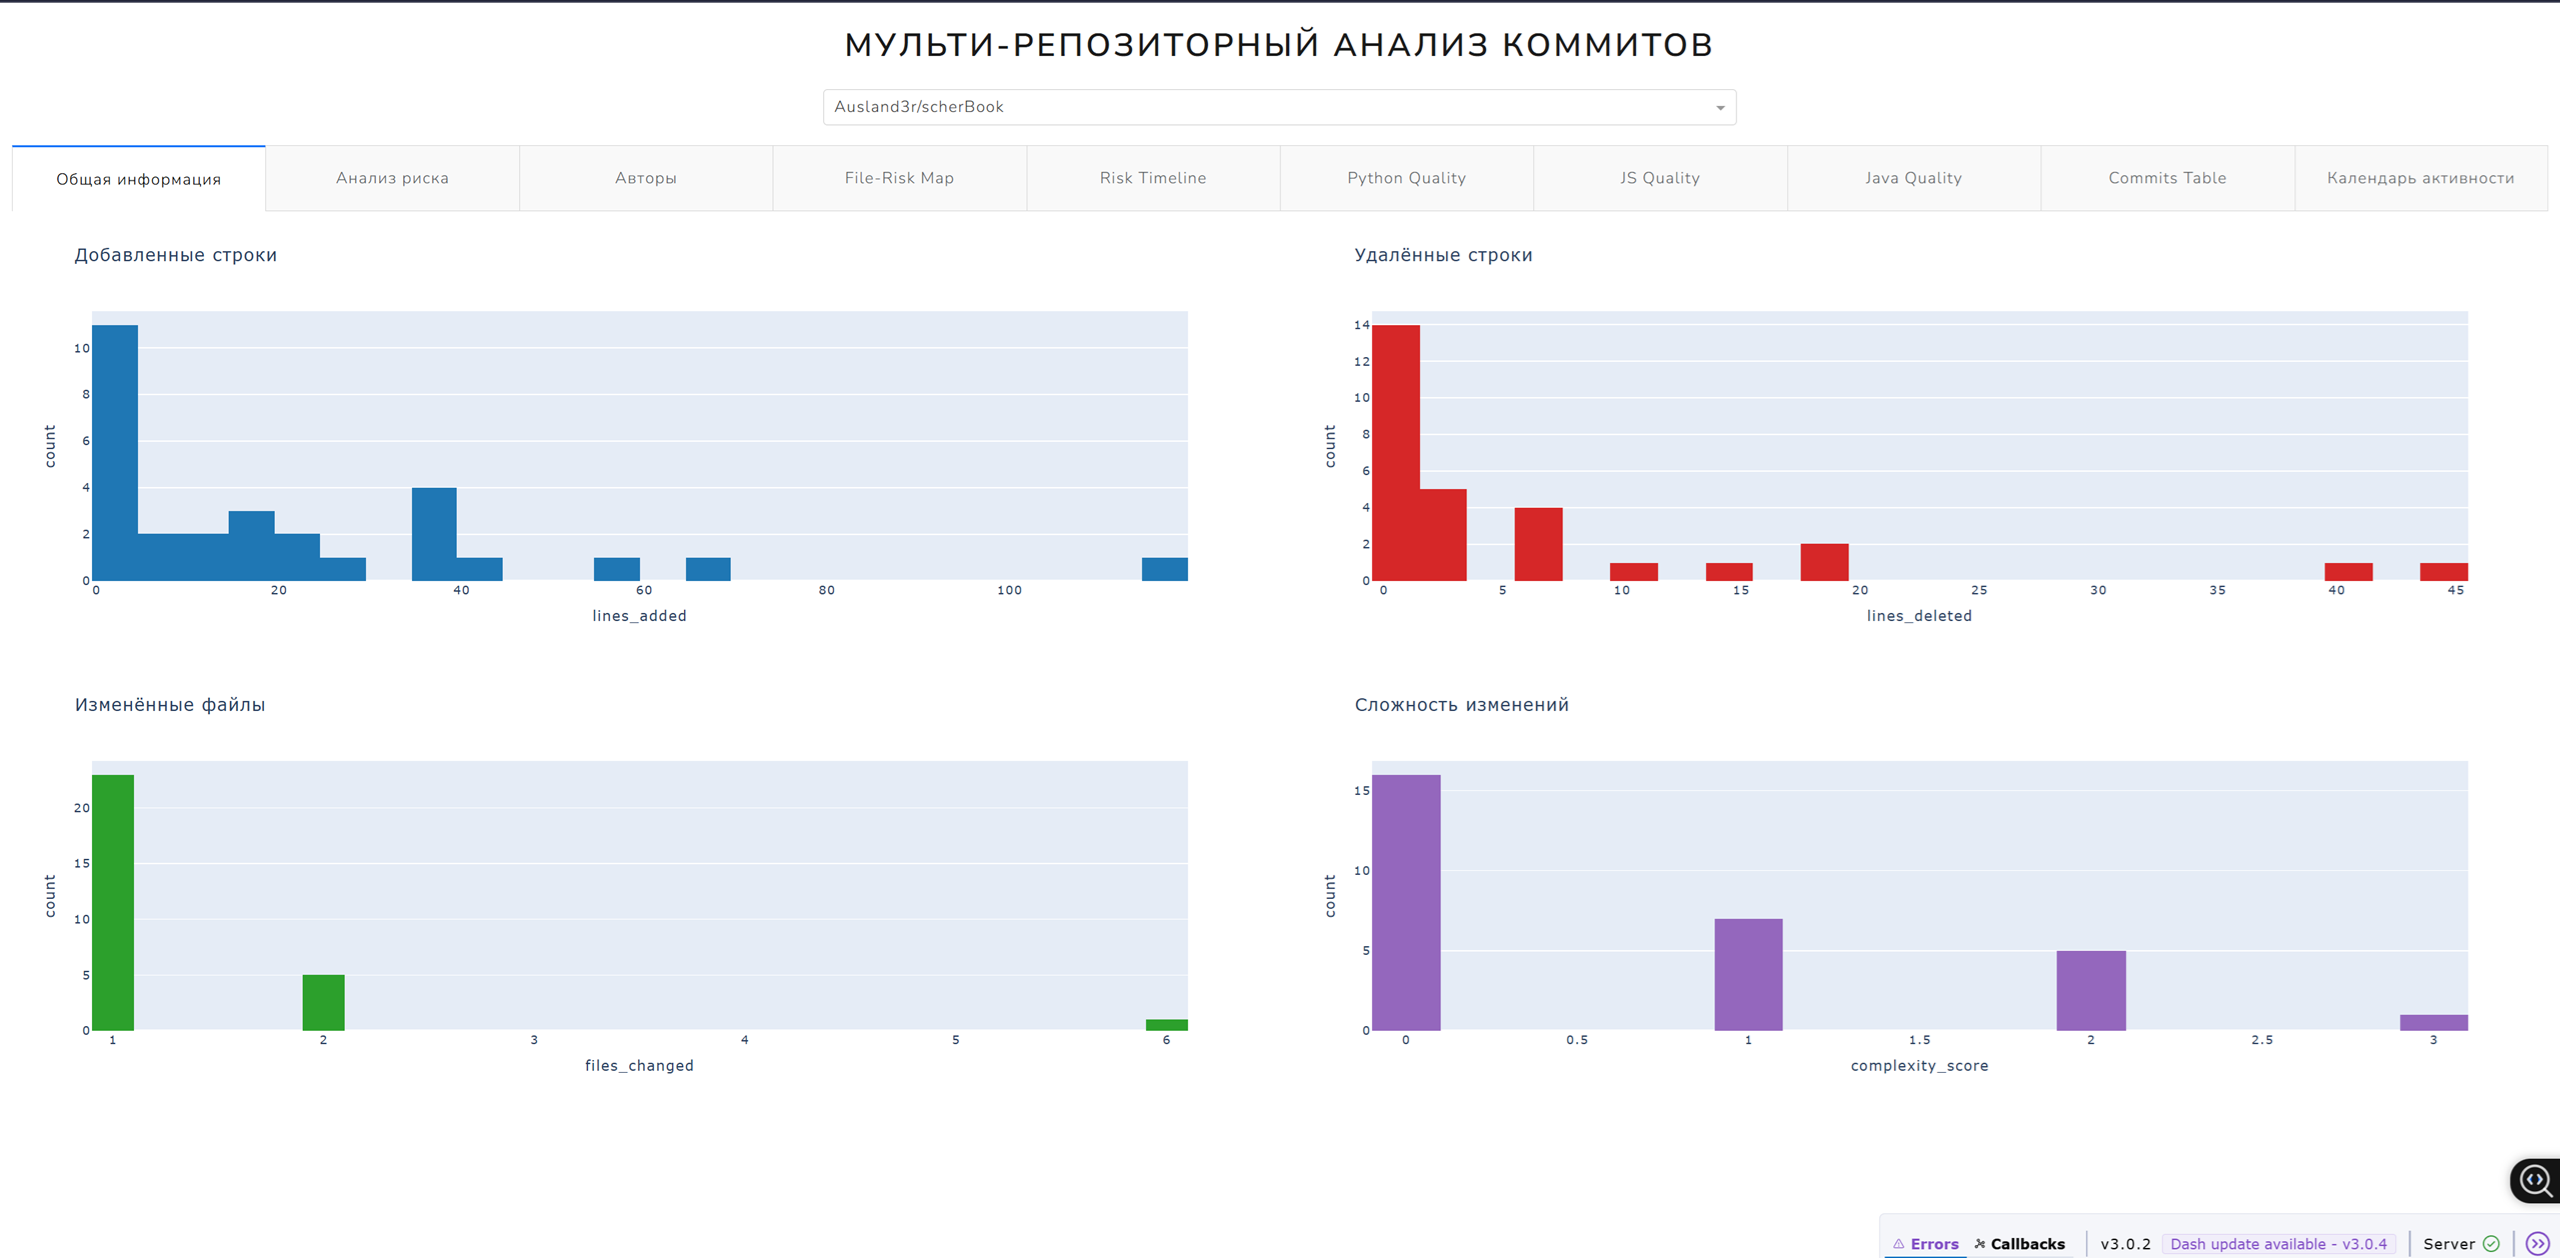
\includegraphics[width=0.85\textwidth]{my_folder/images/dashboard.png}
	\caption{Пример страницы дашборда с общей статистикой по репозиторию}
\end{figure}

\subsection{Пример построения гистограммы с использованием plotly.express}

Для визуализации распределения числовых метрик широко используется компонент \texttt{dcc.Graph} в связке с \texttt{plotly.express}. Например, построение гистограммы по числу добавленных строк реализуется следующим образом:

\begin{lstlisting}[language=Python, caption={Построение гистограммы добавленных строк}]
	dcc.Graph(
	figure=px.histogram(
	df, # DataFrame с данными коммитов
	x = 'lines_added', #По оси X - число добавленных строк
	nbins=30, # Количество корзин гистограммы
	title='Добавленные строки',
	color_discrete_sequence=['#1f77b4']  # Цвет столбцов (синий)
	)
	)
\end{lstlisting}

Такой подход позволяет быстро создавать красивые и информативные графики с минимальными усилиями.

\subsection{Динамическое обновление интерфейса и фильтрация данных}

Для обеспечения интерактивности и гибкости отображения данных в панели используются callback-функции Dash. Они реагируют на действия пользователя, такие как выбор репозитория, фильтрация по авторам или выбор временного диапазона, и динамически обновляют содержимое вкладок и графиков.

Ниже приведён пример callback-функции, которая обновляет вкладки с аналитикой при смене выбранного репозитория в выпадающем списке:

\begin{lstlisting}[language=Python, caption={Callback-функция обновления вкладок по выбранному репозиторию}]
	@app.callback(
	Output("tabs-container", "children"),
	Input("repo-selector", "value")
	)
	def update_tabs(selected_repo):
	if not selected_repo or selected_repo not in analyses:
	return html.Div("Репозиторий не выбран или недоступен")
	
	entry = analyses[selected_repo]
	df = entry['df']
	feat_imps = entry['feat_imps']
	model = entry['model']
	
	# Формирование вкладок с графиками и таблицами на основе выбранного репозитория
	tabs = [
	create_summary_tab(df),
	create_risk_analysis_tab(df, feat_imps, model.features),
	create_authors_tab(df),
	create_file_risk_map_tab(df),
	create_risk_timeline_tab(df),
	create_quality_tabs(df),
	create_commits_table_tab(df),
	create_activity_calendar_tab(df)
	]
	return dcc.Tabs(tabs)
\end{lstlisting}

В этом примере:

\begin{itemize}
	\item \texttt{@app.callback} связывает функцию \texttt{update\_tabs} с изменением значения в выпадающем списке с id \texttt{"repo-selector"}.
	\item Функция получает выбранный репозиторий, извлекает из предобработанных данных соответствующий набор аналитики.
	\item Возвращается обновлённый набор вкладок, которые отображаются в контейнере с id \texttt{"tabs-container"}.
\end{itemize}

Такой подход позволяет пользователю мгновенно переключаться между проектами и получать актуальную аналитику без перезагрузки страницы. Подобным образом можно реализовать и другие callback-функции для фильтрации по авторам, датам и т.д., обеспечивая гибкое и удобное взаимодействие с дашбордом.

\subsection{Генерация и отображение рекомендаций CAPA}

Для каждого коммита в системе формируются рекомендации корректирующих и предупреждающих действий на основе вычисленной вероятности риска и значений метрик. Логика генерации рекомендаций реализована в отдельном модуле \texttt{recommendations.py}, что обеспечивает модульность и упрощает расширение.


Пример функции генерации рекомендаций:

\begin{lstlisting}[language=Python, caption={Пример генерации рекомендаций CAPA}]
	def generate_recommendations(commit, risk_proba, repo_stats, feature_importances):
	recommendations = []
	if risk_proba > 0.8:
	recommendations.append("Очень высокий риск: провести углублённое ревью.")
	if commit['lines_added'] > 100:
	recommendations.append("Большой объём изменений: рекомендуется более тщательное тестирование.")
	return recommendations
\end{lstlisting}

Рекомендации выводятся в таблице коммитов, что облегчает восприятие и принятие решений командой разработчиков.

\section{Интеграция компонентов в единую систему} \label{ch3:sec5}

Вся система реализована как последовательный конвейер обработки данных, объединяющий сбор, анализ, генерацию рекомендаций и визуализацию:

\begin{enumerate}
	\item Сбор и предварительная обработка — модуль \texttt{GitHubRepoAnalyzer} получает из GitHub историю коммитов, локально анализирует содержимое файлов и формирует набор признаков для каждого коммита.
	\item Обучение и применение модели — класс \texttt{CommitRiskModel} обучается на полученных данных, используя псевдометки, после чего применяется для оценки риска новых коммитов.
	\item Генерация рекомендаций — на основе результатов классификации формируются конкретные CAPA для каждого коммита, учитывая статистику репозитория и важность признаков.
	\item Визуализация — все метрики, прогнозы и рекомендации выводятся в веб-интерфейсе Dash, обеспечивая пользователю удобный доступ к аналитике.
	\item Автоматизация — реализован механизм периодического обновления данных, переобучения модели и актуализации интерфейса без участия пользователя.
\end{enumerate}

\begin{figure}[ht!]
	\centering
	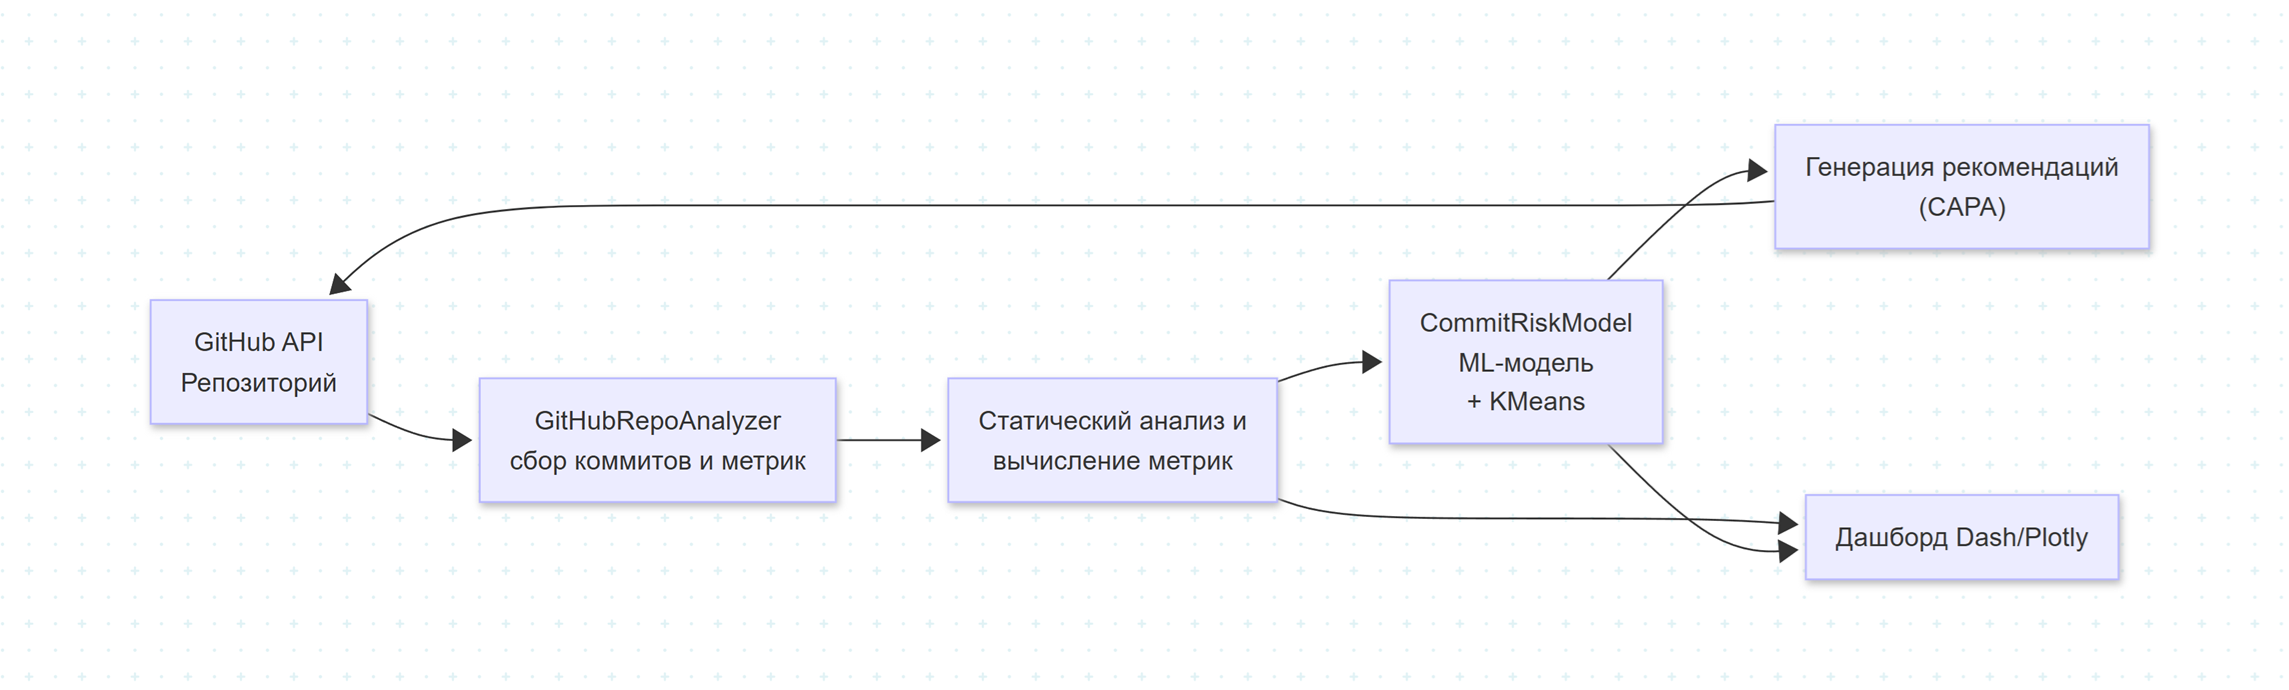
\includegraphics[width=1.1\textwidth]{my_folder/images/mermaid.png}
	\caption{Пайплайн автоматического анализа коммитов GitHub}
	\label{fig:architecture1}
\end{figure}

На диаграмме \ref{fig:architecture1} представлена общая архитектура системы, где чётко прослеживается поток данных: от исходного кода в GitHub через модули анализа и обучения модели до визуализации и генерации CAPA.

\section{Выводы} \label{ch3:sec6}

Реализованная система обеспечивает полный цикл автоматического мониторинга качества разработки на основе анализа коммитов, объединяя в себе сбор данных, интеллектуальную оценку риска и удобную визуализацию. Модульная архитектура позволяет легко расширять функциональность и адаптировать систему под различные проекты.
